
\section{Landasan Metode Runge-Kutta\label{sec:Runge-Kutta-Methods}\index{metode Runge-Kutta}\index{metode!Runge-Kutta|see {metode Runge-Kutta}}}

Dalam bagian \ref{sec:TaylorMethods}, turunan digunakan untuk menghasilkan
solusi aproksimasi persamaan diferensial biasa. Namun, solusi aproksimasi
juga dapat dihasilkan melalui integrasi, suatu proses numerik yang
jauh lebih stabil. Sebuah PDB berbentuk
\begin{eqnarray*}
\dot{y} & = & f(t,y)\\
y(t_{0}) & = & y_{0}
\end{eqnarray*}
memiliki solusi eksak yang dapat ditulis dalam bentuk integral. Untuk
sembarang nilai $\tilde{t}$, dan dengan mengasumsikan adanya solusi
pada selang dari $t_{0}$ hingga $\tilde{t}$, kita dapat menentukan
nilai $y(\tilde{t})$ dengan mengintegralkan kedua ruas $\dot{y}=f(t,y)$
terhadap $t$: 
\begin{eqnarray}
\int_{t_{0}}^{\tilde{t}}\dot{y}\,dt & = & \int_{t_{0}}^{\tilde{t}}f(t,y)\,dt\nonumber \\
y(\tilde{t})-y(t_{0}) & = & \int_{t_{0}}^{\tilde{t}}f(t,y)\,dt\nonumber \\
y(\tilde{t}) & = & y(t_{0})+\int_{t_{0}}^{\tilde{t}}f(t,y)\,dt.\label{eq:basicRKidea}
\end{eqnarray}
Ketika $t_{0}$ dan $\tilde{t}$ tidak berdekatan, sebagaimana biasanya
kita asumsikan, kita perlu melanjutkan dengan langkah-langkah kecil
seperti yang dilakukan dalam bagian \ref{sec:TaylorMethods}. 

Dengan menyubstitusikan $t_{1}$ untuk menggantikan $\tilde{t}$ dalam
persamaan \ref{eq:basicRKidea}, diperoleh $y(t_{1})=y(t_{0})+\int_{t_{0}}^{t_{1}}f(t,y)\,dt$,
sehingga kita dapat menambahkan $\int_{t_{0}}^{t_{1}}f(t,y)\,dt$
pada nilai yang telah diketahui $y(t_{0})$ untuk memperoleh $y(t_{1})$,
langkah kecil pertama dalam proses mengaproksimasi $y(\tilde{t})$.
Selanjutnya, dengan menyubstitusikan $t_{1}$ untuk menggantikan $t_{0}$
dan $t_{2}$ untuk menggantikan $\tilde{t}$ dalam persamaan \ref{eq:basicRKidea},
diperoleh $y(t_{2})=y(t_{1})+\int_{t_{1}}^{t_{2}}f(t,y)\,dt$. Dengan
demikian, kita dapat menghitung $y(t_{2})$ berdasarkan nilai $y(t_{1})$.
Dengan cara serupa, kita dapat menghitung $y(t_{3})$ berdasarkan
nilai $y(t_{2})$, $y(t_{4})$ berdasarkan nilai $y(t_{3})$, dan
seterusnya, hingga akhirnya menghitung $y(t_{n})=y(\tilde{t})$. Dengan
mengingat hal ini, kita menulis ulang representasi integral dalam
bentuk $t_{i}$ dan $t_{i+1}$ alih-alih $t_{0}$ dan $\tilde{t}$:
\begin{equation}
y(t_{i+1})=y(t_{i})+\int_{t_{i}}^{t_{i+1}}f(t,y)\,dt.\label{eq:integralEquation}
\end{equation}
Rumus ini menunjukkan bahwa memperoleh satu nilai aproksimasi, $y(t_{i+1})$,
dari nilai sebelumnya, $y(t_{i})$, pada dasarnya cukup dengan mengaproksimasi
$\int_{t_{i}}^{t_{i+1}}f(t,y)\,dt$. Hal tersebut seharusnya tidak
terlalu sulit pada tahap ini. Sekitar separuh bab \ref{chap:Numerical-Calculus}
dikhususkan tepat untuk tugas ini! Setiap rumus integrasi numerik
dapat digunakan di sini, tetapi mari kita mulai dari yang sederhana.
Kita mengetahui $y(t_{i})$, yaitu nilai fungsi di titik ujung kiri
integrasi, setidaknya secara aproksimasi, sehingga masuk akal untuk
menggunakan stensil yang memuat titik ujung kiri integrasi sebagai
salah satu simpulnya. Agar percobaan pertama kita sesederhana mungkin,
mari jadikan simpul itu satu-satunya simpul! Dengan kata lain, mari
kita tentukan rumus integrasi untuk stensil

\begin{center}
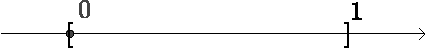
\includegraphics{figures/ode-rungekutta01}.
\par\end{center}

\noindent Dengan metode koefisien tak tentu, kita menghitung ruas
kiri sistem \ref{eq:systemGenericIntegral} (yang bagi kita hanya
terdiri atas satu persamaan karena hanya ada satu simpul):
\begin{eqnarray*}
\int_{a}^{b}p_{0}(x)dx=\int_{x_{0}}^{x_{0}+h}p_{0}(x)dx & = & \int_{x_{0}}^{x_{0}+h}1dx=\left.(x-x_{0})\right|_{x_{0}}^{x_{0}+h}=h
\end{eqnarray*}
dan ruas kanan:
\[
\sum_{i=0}^{0}(\theta_{i}h)^{0}a_{i}=a_{0}.
\]
Jadi $a_{0}=h$ dan kita memperoleh rumus 
\[
\int_{x_{0}}^{x_{0}+h}f(x)dx\approx hf(x_{0}).
\]
Akibatnya, $\int_{t_{i}}^{t_{i+1}}f(t,y)\,dt\approx(t_{i+1}-t_{i})f(t_{i},y(t_{i}))$,
dan persamaan \ref{eq:integralEquation} menjadi
\[
y(t_{i+1})=y(t_{i})+f(t_{i},y(t_{i}))\cdot(t_{i+1}-t_{i}).
\]
Dengan menggunakan notasi $y_{i}=y(t_{i})$ dan $f=\dot{y}$ dari
bagian \ref{sec:TaylorMethods}, rumus ini menjadi
\[
y_{i+1}=y_{i}+\dot{y}(t_{i},y_{i})\cdot(t_{i+1}-t_{i}).
\]
Tunggu sebentar! Kita pernah melihatnya. Ini tepat sama dengan persamaan
\ref{eq:EulersMethodGeneral}.

Pencarian metode baru untuk mengaproksimasi solusi PDB melalui integrasi
sejauh ini belum menghasilkan sesuatu yang baru. Namun, mestinya ada
perbedaan. Rumus integrasi mencakup penghitungan nilai integran di
berbagai titik, sedangkan metode Taylor mencakup penghitungan nilai
turunan di satu titik. Mari kita lanjutkan. Barangkali rumus integrasi
paling sederhana berikutnya yang memuat titik ujung kiri integrasi
adalah Aturan Trapesium (lihat bagian \ref{sec:calculusErrorAnalysis}),
\[
{\displaystyle \int_{x_{0}}^{x_{0}+h}f(x)dx=\frac{h}{2}\left[f(x_{0})+f(x_{0}+h)\right]+O(h^{3}f''(\xi_{h}))}
\]
pada stensil

\begin{center}
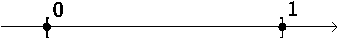
\includegraphics[scale=1.67]{figures/ode-rungekutta13}.
\par\end{center}

\noindent Dengan menerjemahkan Aturan Trapesium ke dalam notasi saat
ini,
\[
{\displaystyle \int_{t_{i}}^{t_{i+1}}f(t,y)\,dt=\frac{t_{i+1}-t_{i}}{2}\left[f(t_{i},y_{i})+f(t_{i+1},y_{i+1})\right]+O((t_{i+1}-t_{i})^{3}).}
\]
Dengan demikian, rumus aproksimasi baru kita adalah
\[
y_{i+1}=y_{i}+\frac{t_{i+1}-t_{i}}{2}\left[f(t_{i},y_{i})+f(t_{i+1},y_{i+1})\right].
\]
Persamaan ini sangat baik, kecuali bahwa ruas kanannya memuat $y_{i+1}$,
yaitu besaran yang sedang kita aproksimasi! Salah satu pilihan adalah
membiarkannya demikian. Persamaan untuk $y_{i+1}$ bersifat implisit,
dan itu tidak menjadi masalah. Suatu metode pencarian akar dapat digunakan
untuk menentukan $y_{i+1}$ pada setiap langkah metode tersebut. Meskipun
cara ini bukan tidak mungkin, cara ini juga bukan solusi yang paling
sederhana. Karena ukuran langkah $(t_{i+1}-t_{i})$ kemungkinan kecil,
barangkali penggunaan metode Euler untuk mengaproksimasi $y_{i+1}$
di ruas kanan tidak akan menimbulkan kerusakan yang tak dapat diperbaiki
pada aproksimasi keseluruhan. Untuk mencobanya, kita gunakan $y_{i+1}=y_{i}+(t_{i+1}-t_{i})\cdot f(t_{i},y_{i})$
di ruas kanan untuk memperoleh rumus baru 
\[
y_{i+1}=y_{i}+\frac{t_{i+1}-t_{i}}{2}\left[f(t_{i},y_{i})+f(t_{i+1},y_{i}+(t_{i+1}-t_{i})\cdot f(t_{i},y_{i}))\right].
\]
Sejenak mempertimbangkan hasil kita, mungkin kita menyimpulkan bahwa
rumus tersebut mulai agak rumit. Mari kita lihat apakah rumus tersebut
dapat sedikit dirapikan. Pertama, menyubstitusikan $h$ untuk menggantikan
$t_{i+1}-t_{i}$ membuatnya sedikit lebih sederhana:
\[
y_{i+1}=y_{i}+\frac{h}{2}\left[f(t_{i},y_{i})+f(t_{i+1},y_{i}+h\cdot f(t_{i},y_{i}))\right].
\]
Kedua, dengan menetapkan $k_{1}=f(t_{i},y_{i})$ dan $k_{2}=f(t_{i+1},y_{i}+h\cdot f(t_{i},y_{i}))=f(t_{i+1},y_{i}+h\cdot k_{1})$,
kita memperoleh perhitungan tiga langkah yang rapi dan ringkas:
\begin{eqnarray}
k_{1} & = & f(t_{i},y_{i})\nonumber \\
k_{2} & = & f(t_{i+1},y_{i}+hk_{1})\nonumber \\
y_{i+1} & = & y_{i}+\frac{h}{2}(k_{1}+k_{2}).\label{eq:trapezoidal-ode}
\end{eqnarray}
Namun, sebelum terlalu terbawa oleh rumusan yang rapi ini, sebaiknya
kita mencari beberapa bukti bahwa metode ``canggih'' ini memberikan
aproksimasi yang masuk akal bagi solusi suatu PDB sebagaimana diharapkan.
Mari kita minta Octave menghitung solusi aproksimasi PDB \ref{eq:sampleODE}
dengan metode Euler maupun metode berbasis Aturan Trapesium ini, lalu
membandingkannya dengan solusi eksak, $y(t)=\frac{t^{3}}{4}+\frac{16}{t}$.
Cuplikan kode berikut, meskipun khusus untuk tugas ini, dapat digeneralisasi
untuk menentukan solusi aproksimasi PDB lainnya.

\subsubsection{Kode uji pemecah PDB}
\begin{lyxcode}
t=4;

h=-1/4;

f=@(t,y)~-y/t+t\textasciicircum 2;

exact=@(t)~t\textasciicircum 3/4+16/t;

euler=20;

trap=20;

disp('~~~~~~~~~~~~~Euler~~~Trapezoid~~~~~~~Exact~~~Euler~err~~~~Trap~err')

disp('~~~~~~~~-{}-{}-{}-{}-{}-{}-{}-{}-{}-{}-{}-{}-{}-{}-{}-{}-{}-{}-{}-{}-{}-{}-{}-{}-{}-{}-{}-{}-{}-{}-{}-{}-{}-{}-{}-{}-{}-{}-{}-{}-{}-{}-{}-{}-{}-{}-{}-{}-{}-{}-{}-{}-{}-{}-{}-{}-{}-{}-{}-{}-')

for~i=1:8

~~euler=euler+h{*}f(t,euler);

~~k1=f(t,trap);

~~k2=f(t+h,trap+h{*}k1);

~~trap=trap+h/2{*}(k1+k2);

~~t=t+h;

~~x=exact(t);

~~sprintf('\%12.5g\%12.5g\%12.5g\%12.5g\%12.5g',euler,trap,x,abs(euler-x),abs(trap-x))

end\%for
\end{lyxcode}
Kode uji ini dapat diunduh dari \href{http://lqbrin.github.io/tea-time-numerical/ancillaries.html}{situs pendamping}
(\texttt{rungeKuttaDemo.m}). Satu-satunya bagian kode ini yang mungkin
terasa asing bagi Anda pada tahap ini adalah perintah \texttt{sprintf()}
tersebut. \index{Octave!sprintf@\texttt{sprintf}} Argumen pertama,

\begin{center}
\texttt{'\%12.5g\%12.5g\%12.5g\%12.5g\%12.5g'}, 
\par\end{center}

\noindent adalah untai format. Untai ini berarti merangkai 5 bilangan
titik-mengambang dengan masing-masing 12 spasi dan menampilkan 5 angka
signifikan. Dalam perintah \texttt{sprintf}, \texttt{\%12.5g} berarti
pemformatan ``umum'' bagi bilangan titik-mengambang dengan 12 spasi
dan 5 angka signifikan. Komputer akan menentukan apakah notasi ilmiah
digunakan dalam keluaran. Karena diulang 5 kali, perintah ini akan
memformat lima nilai titik-mengambang semacam itu. Argumen lainnya
adalah lima bilangan yang akan dicetak. Perintah \texttt{sprintf}
sebaiknya tidak dibaca sebagai ``sprint-eff'' melainkan ``ess-print-eff''
atau ``string print formatted''. Huruf \texttt{s} menyatakan untai,
sedangkan huruf \texttt{f} menyatakan pemformatan. Jika Anda berpikir
bahwa perintah ini terasa agak rumit, Anda benar. Jenis perintah pemformatan
cetak ini berasal dari bahasa pemrograman C pada tahun 1970-an!\cprotect\footnote{Lihat \url{https://en.wikipedia.org/wiki/Printf_format_string} untuk
beberapa rinciannya.} Keluaran dari menjalankan kode Octave ini adalah
\begin{lyxcode}
~~~~~~~~~~~~~Euler~~~Trapezoid~~~~~~~Exact~~~Euler~err~~~~Trap~err

~~~~~~~~-{}-{}-{}-{}-{}-{}-{}-{}-{}-{}-{}-{}-{}-{}-{}-{}-{}-{}-{}-{}-{}-{}-{}-{}-{}-{}-{}-{}-{}-{}-{}-{}-{}-{}-{}-{}-{}-{}-{}-{}-{}-{}-{}-{}-{}-{}-{}-{}-{}-{}-{}-{}-{}-{}-{}-{}-{}-{}-{}-{}-

ans~=~~~~~~~~17.25~~~~~~17.442~~~~~~~17.45~~~~~0.20026~~~0.0080729

ans~=~~~~~~~14.884~~~~~~15.273~~~~~~~15.29~~~~~~0.4058~~~~0.016741

ans~=~~~~~~~12.885~~~~~~13.479~~~~~~13.505~~~~~0.62006~~~~0.026142

ans~=~~~~~~~11.236~~~~~~12.047~~~~~~12.083~~~~~0.84776~~~~0.036458

ans~=~~~~~~~9.9219~~~~~~10.969~~~~~~11.017~~~~~~1.0955~~~~~0.04794

ans~=~~~~~~~8.9332~~~~~~10.245~~~~~~10.306~~~~~~~1.373~~~~0.060938

ans~=~~~~~~~8.2641~~~~~~9.8828~~~~~~9.9588~~~~~~1.6947~~~~0.075955

ans~=~~~~~~~7.9167~~~~~~9.9062~~~~~~~~~~10~~~~~~2.0833~~~~~0.09375
\end{lyxcode}
Metode kita yang didasarkan pada Aturan Trapesium, yang akan kita
sebut PDB-trapesium untuk sementara, tampaknya lebih baik dalam menghampiri
solusi PDB ini daripada metode Euler. Dua kolom terakhir memuat galat
absolut untuk setiap hampiran. Galat pada PDB-trapesium kira-kira
0.01 hingga 0.1, sedangkan galat pada metode Euler kira-kira 0.2 hingga
2. Semua galat pada PDB-trapesium lebih kecil daripada semua galat
pada metode Euler. Tentu saja, PDB-trapesium memerlukan dua evaluasi
$f$ per langkah, sehingga metode itu seharusnya memberikan hasil
lebih baik yang sepadan dengan upaya tambahan tersebut jika hendak
berguna.

Terdorong oleh keberhasilan ini, mungkin ada baiknya meluangkan waktu
untuk rumus integrasi lain, misalnya Aturan Simpson. Ingat kembali
dari bagian \ref{sec:calculusErrorAnalysis}, Aturan Simpson menyatakan
\[
{\displaystyle \int_{x_{0}}^{x_{0}+2h}f(x)dx=\frac{h}{3}\left[f(x_{0})+4f(x_{0}+h)+f(x_{0}+2h)\right]+O(h^{5}f^{(4)}(\xi_{h}))},
\]
yang dalam notasi bagian ini dapat kita tulis sebagai
\[
\int_{t_{i}}^{t_{i+1}}f(t,y)\,dt=\frac{h}{6}\left[f(t_{i},y_{i})+4f(t_{i+1/2},y_{i+1/2})+f(t_{i+1},y_{i+1})\right],
\]
dengan mengabaikan suku galat dan menggunakan notasi $t_{i+1/2}$
untuk menyatakan $t_{i}+\frac{1}{2}h$ dan $y_{i+1/2}$ untuk menyatakan
$y(t_{i}+\frac{1}{2}h)$. Jadi, penyelesai PDB yang didasarkan pada
Aturan Simpson dapat berbentuk
\[
y_{i+1}=y_{i}+\frac{h}{6}\left[f(t_{i},y_{i})+4f(t_{i+1/2},y_{i+1/2})+f(t_{i+1},y_{i+1})\right].
\]
Sekali lagi, ini adalah rumus implisit. Sekali lagi, kita dapat menggunakan
metode Euler untuk menaksir $y_{i+1}$, dan bahkan kita dapat menggunakan
metode Euler untuk menaksir $y_{i+1/2}$ juga! Karena $t_{i+1/2}$
lebih dekat ke $t_{i}$ daripada $t_{i+1}$, kita menaksir $y_{i+1/2}$
terlebih dahulu. Artinya, kita mengganti $y_{i+1/2}$ dengan $y_{i}+\frac{h}{2}f(t_{i},y_{i})$.
Dengan perhitungan dalam beberapa langkah seperti sebelumnya, kita
memperoleh
\begin{eqnarray*}
k_{1} & = & f(t_{i},y_{i})\\
k_{2} & = & f\left(t_{i}+\frac{h}{2},y_{i}+\frac{h}{2}k_{1}\right)
\end{eqnarray*}
sampai tahap ini. Ini menangani dua suku pertama di dalam tanda kurung
siku. Sekarang kita menaksir $y_{i+1}$ dengan menghampiri $f(t_{i+1},y_{i+1})$.
Namun, sekarang kita memiliki taksiran untuk $f$ pada $t_{i}+\frac{h}{2}$,
dan $t_{i}+\frac{h}{2}$ lebih dekat ke $t_{i+1}$ daripada $t_{i}$.
Jadi, meskipun kita dapat menggunakan $y_{i}+hf(t_{i},y_{i})=y_{i}+hk_{1}$
untuk menghampiri $y_{i+1}$ (seperti yang dilakukan sebelumnya),
kita dapat menduga bahwa $y_{i}+hk_{2}$ merupakan taksiran yang lebih
baik. Dengan harapan ini, kita menyelesaikan metode tersebut melalui
perhitungan berikut:
\begin{eqnarray*}
k_{1} & = & f(t_{i},y_{i})\\
k_{2} & = & f\left(t_{i}+\frac{h}{2},y_{i}+\frac{h}{2}k_{1}\right)\\
k_{3} & = & f(t_{i+1},y_{i}+hk_{2})\\
y_{i+1} & = & y_{i}+\frac{h}{6}\left[k_{1}+4k_{2}+k_{3}\right].
\end{eqnarray*}
Untuk sementara, kita akan menyebut metode ini PDB-Simpson. 

Sebelum mencoba menilai apakah metode baru ini lebih baik daripada
metode-metode sebelumnya, mari kita turunkan beberapa metode lagi
dan membandingkan semuanya sekaligus. Rumus
\[
{\displaystyle \int_{x_{0}}^{x_{0}+3h}f(x)dx=\frac{3h}{2}\left[f(x_{0}+h)+f(x_{0}+2h)\right]+O(h^{3}f''(\xi_{h}))}
\]
 (sebuah rumus Newton-Cotes terbuka dari bagian \ref{sec:calculusErrorAnalysis})
menghasilkan metode
\begin{eqnarray*}
k_{1} & = & f(t_{i},y_{i})\\
k_{2} & = & f\left(t_{i}+\frac{h}{3},y_{i}+\frac{h}{3}k_{1}\right)\\
k_{3} & = & f\left(t_{i}+\frac{2h}{3},y_{i}+\frac{2h}{3}k_{2}\right)\\
y_{i+1} & = & y_{i}+\frac{h}{2}\left[k_{2}+k_{3}\right].
\end{eqnarray*}
Dapatkah Anda melengkapi langkah-langkah untuk menurunkan metode ini?
Jawaban \vpageref{ans:fill-in}. Kita akan menyebut metode ini PDB-terbuka.
Terakhir, kita menggunakan stensil

\begin{center}
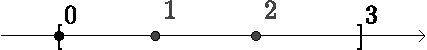
\includegraphics{figures/ode-rungekutta02}
\par\end{center}

\noindent untuk menurunkan rumus integrasi lainnya. Rumus ini bukan
rumus Newton-Cotes terbuka dan juga bukan rumus Newton-Cotes tertutup.
Rumus ini tidak dibahas dalam bagian \ref{sec:calculusErrorAnalysis}.
Mungkin rumus ini dapat disebut rumus Newton-Cotes ``tertutup-terbuka''
(setengah tertutup dan setengah terbuka). Dapatkah Anda menurunkan
metode integrasi yang bersesuaian? Rincian \vpageref{ans:clopenNewtonCotes}.
Hasilnya adalah
\[
\int_{x_{0}}^{x_{0}+3h}f(x)dx\approx\frac{3h}{4}\left[f(x_{0})+3f(x_{0}+2h)\right],
\]
dengan mengabaikan suku galat. Hal ini menghasilkan penyelesai PDB
\begin{eqnarray*}
k_{1} & = & f(t_{i},y_{i})\\
k_{2} & = & f\left(t_{i}+\frac{h}{3},y_{i}+\frac{h}{3}k_{1}\right)\\
k_{3} & = & f\left(t_{i}+\frac{2h}{3},y_{i}+\frac{2h}{3}k_{2}\right)\\
y_{i+1} & = & y_{i}+\frac{h}{4}\left[k_{1}+3k_{3}\right].
\end{eqnarray*}
Kita akan menyebut metode ini PDB-tertutup-terbuka. Perhatikan dua
hal. Pertama, meskipun $k_{2}$ tidak digunakan pada baris terakhir,
nilai tersebut tetap dihitung karena digunakan untuk menghitung $k_{3}$.
Kedua, perhitungan $k_{1}$, $k_{2}$, dan $k_{3}$ identik dengan
perhitungan dalam metode PDB-terbuka. Satu-satunya perbedaan terletak
pada cara $k_{j}$ digabungkan. Metode integrasi tersebut menggabungkan
nilai fungsi pada simpul dengan cara berbeda. Gagasan menggunakan
$k_{j}$ yang sama untuk tujuan berbeda akan muncul lagi!

Jadi, kini kita memiliki tiga metode baru untuk diuji---satu didasarkan
pada Aturan Simpson (PDB-Simpson), satu didasarkan pada rumus Newton-Cotes
terbuka (PDB-terbuka), dan yang ketiga didasarkan pada rumus Newton-Cotes
yang disebut ``tertutup-terbuka'' (PDB-tertutup-terbuka). Dapatkah
Anda menulis kode uji untuk membandingkan ketiga rumus baru tersebut
(serupa dengan kode yang digunakan untuk membandingkan metode Euler
dengan PDB-trapesium)? Jawaban \vpageref{ans:testCode}. Hasilnya
dirangkum dalam keluaran Octave berikut:
\begin{lyxcode}
~~~~~~~~Simpsons~~Open~~~~~~Clopen~~~~Simp~err~~Open~err~~Clop~err

~~~~~~~~-{}-{}-{}-{}-{}-{}-{}-{}-{}-{}-{}-{}-{}-{}-{}-{}-{}-{}-{}-{}-{}-{}-{}-{}-{}-{}-{}-{}-{}-{}-{}-{}-{}-{}-{}-{}-{}-{}-{}-{}-{}-{}-{}-{}-{}-{}-{}-{}-{}-{}-{}-{}-{}-{}-{}-{}-{}-{}-{}-

ans~=~~~17.44806~~17.44999~~17.45022~~~0.00220~~~0.00028~~~0.00004

ans~=~~~15.28557~~15.28953~~15.29008~~~0.00461~~~0.00065~~~0.00010

ans~=~~~13.49781~~13.50395~~13.50494~~~0.00730~~~0.00116~~~0.00017

ans~=~~~12.07297~~12.08146~~12.08307~~~0.01036~~~0.00187~~~0.00027

ans~=~~~11.00347~~11.01450~~11.01700~~~0.01393~~~0.00290~~~0.00040

ans~=~~~10.28804~~10.30185~~10.30566~~~0.01821~~~0.00440~~~0.00059

ans~=~~~~9.93523~~~9.95208~~~9.95789~~~0.02354~~~0.00669~~~0.00088

ans~=~~~~9.96952~~~9.98969~~~9.99866~~~0.03048~~~0.01031~~~0.00134
\end{lyxcode}
PDB-Simpson paling buruk dalam memperoleh solusi aproksimasi, sedangkan
PDB-tertutup-terbuka paling baik. Namun, mengapa?

Hingga saat ini, kita telah cukup menyeluruh dalam mengesampingkan
analisis galat. Bagian terbesar penyelidikan tersebut akan dilakukan
pada bagian berikutnya, tetapi kita dapat melakukan analisis singkat
di sini. Dari bagian \ref{sec:calculusErrorAnalysis}, kita mengetahui
bahwa Aturan Trapesium dan rumus Newton-Cotes terbuka yang kita gunakan
di sini sama-sama memiliki suku galat $O(h^{3})$, sedangkan Aturan
Simpson memiliki suku galat $O(h^{5})$. Metode integrasi yang didasarkan
pada stensil

\begin{center}
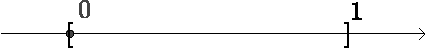
\includegraphics{figures/ode-rungekutta01}
\par\end{center}

\begin{center}
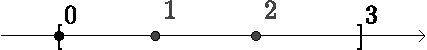
\includegraphics{figures/ode-rungekutta02}
\par\end{center}

\noindent (yang menghasilkan metode Euler dan PDB-tertutup-terbuka)
memiliki suku galat yang belum ditentukan. Dapatkah Anda menunjukkan
bahwa suku galat tersebut masing-masing adalah $O(h^{2})$ dan $O(h^{4})$?
Jawaban \vpageref{ans:errorTerms}. Berdasarkan suku galat metode
integrasi yang mendasarinya, kita memperkirakan bahwa urutan penyelesai
PDB dari yang paling tidak akurat hingga paling akurat adalah metode
Euler (berdasarkan rumus integrasi yang memiliki $O(h^{2})$ sebagai
suku galatnya), PDB-terbuka (berdasarkan rumus integrasi yang memiliki
$O(h^{3})$ sebagai suku galatnya), PDB-tertutup-terbuka (berdasarkan
rumus integrasi yang memiliki $O(h^{4})$ sebagai suku galatnya),
dan PDB-Simpson (berdasarkan rumus integrasi yang memiliki $O(h^{5})$
sebagai suku galatnya); sedangkan PDB-trapesium diperkirakan setara
dengan PDB-terbuka. Tabel \ref{tab:odeCompare} menunjukkan galat
perhitungan $y(2)$ untuk \ref{eq:sampleODE} bagi kelima metode dalam
bagian ini dengan berbagai nilai $h$. 
\begin{table}
\caption{\label{tab:odeCompare}Perbandingan galat absolut untuk lima penyelesai
PDB}

\begin{centering}
\begin{tabular}{cccccc}
$h$ & Euler & PDB-trapesium & PDB-terbuka & PDB-tertutup-terbuka & PDB-Simpson\tabularnewline
\hline 
$-\frac{1}{4}$ & $2.0833$ & $0.09375$ & $0.010311$ & $0.0013444$ & $0.030482$\tabularnewline
$-\frac{1}{8}$ & $1.0809$ & $0.023437$ & $0.0025929$ & $0.00017446$ & $0.0077168$\tabularnewline
$-\frac{1}{16}$ & $0.55114$ & $0.0058594$ & $0.00064977$ & $2.2207(10)^{-5}$ & $0.0019412$\tabularnewline
$-\frac{1}{32}$ & $0.27837$ & $0.0014648$ & $0.00016261$ & $2.8008(10)^{-6}$ & $0.00048679$\tabularnewline
$-\frac{1}{64}$ & $0.1399$ & $0.00036621$ & $4.0672(10)^{-5}$ & $3.5166(10)^{-7}$ & $0.00012188$\tabularnewline
$-\frac{1}{128}$ & $0.07013$ & $9.1553(10)^{-5}$ & $1.017(10)^{-5}$ & $4.4055(10)^{-8}$ & $3.0494(10)^{-5}$\tabularnewline
\end{tabular}
\par\end{centering}
\end{table}
Karena nilai $h$ pada setiap baris adalah setengah dari nilai pada
baris sebelumnya, kita memperkirakan rasio galat pada baris berurutan
kira-kira $\left(\frac{1}{2}\right)^{\ell}$ jika laju kekonvergenan
metode tersebut adalah $O(h^{\ell})$. Untuk metode Euler, dengan
membagi galat pada baris 3 dengan galat pada baris 2, kita memperoleh
$\left(\frac{1}{2}\right)^{\ell}\approx\frac{.55114}{1.0809}\approx\frac{1}{2}$
dan dengan membagi galat pada baris 6 dengan galat pada baris 5, kita
memperoleh $\left(\frac{1}{2}\right)^{\ell}\approx\frac{.07013}{.1399}\approx\frac{1}{2}$,
misalnya. Bukti ini menunjukkan bahwa $\ell=1$ untuk metode Euler
dan, oleh karena itu, metode Euler memiliki sifat $O(h)$ dalam kekonvergenannya.
Mengulangi perhitungan yang sama untuk metode lain menghasilkan Tabel
\ref{tab:odeMethodOrders}.
\begin{table}
\caption{\label{tab:odeMethodOrders}Suku galat lima penyelesai PDB dan metode
integrasi yang mendasarinya}

\begin{centering}
\begin{tabular}{cccccc}
 & Euler & PDB-trapesium & PDB-terbuka & PDB-tertutup-terbuka & PDB-Simpson\tabularnewline
\hline 
Metode integrasi & $O(h^{2})$ & $O(h^{3})$ & $O(h^{3})$ & $O(h^{4})$ & $O(h^{5})$\tabularnewline
Penyelesai PDB & $O(h)$ & $O(h^{2})$ & $O(h^{2})$ & $O(h^{3})$ & $O(h^{2})$\tabularnewline
\end{tabular}
\par\end{centering}
\end{table}

Dengan pengecualian PDB-Simpson, Tabel \ref{tab:odeMethodOrders}
menunjukkan bahwa suku galat metode penyelesaian PDB berderajat satu
tingkat lebih rendah daripada rumus integrasi (satu langkah) yang
mendasarinya. Dalam Bagian \ref{sec:Composite} kita mencatat bahwa
rumus integrasi komposit juga memiliki suku galat dengan derajat satu
tingkat lebih rendah daripada rumus integrasi satu langkah yang bersesuaian
(dan kita membuat pengamatan serupa tentang metode Taylor dalam Bagian
\ref{sec:TaylorMethods}). Ada alasan untuk meyakini kesejajaran ini
karena metode-metode yang diajukan dalam bagian ini pada dasarnya
merupakan teknik integrasi komposit. Karena itu, kenyataan bahwa PDB-Simpson
tidak mengikuti pola tersebut seharusnya agak mengkhawatirkan. Kajian
yang lebih mendalam terhadap suku galat diperlukan untuk menjelaskan
anomali ini.

\noindent\begin{small} 

\subsection{Latihan}
\begin{enumerate}
\item \label{exc:ode-rungeKutta}Turunkan metode penyelesaian PDB berdasarkan
stensil dan rumus integrasi yang bersesuaian.

\begin{enumerate}
\item \label{exc:ode-rungeKutta-1}\hasasolution 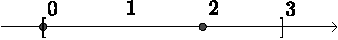
\includegraphics{figures/ode-rungeKutta03}
\[
\frac{h}{4}\left(f(x_{0})+3f\left(x_{0}+\frac{2}{3}h\right)\right)+O(h^{4})
\]
\item \label{exc:ode-rungeKutta-2}\hasananswer 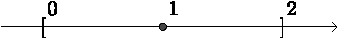
\includegraphics{figures/ode-rungeKutta04}
\[
hf\left(x_{0}+\frac{1}{2}h\right)+O(h^{3})
\]
\item \label{exc:ode-rungeKutta-3}\hasananswer 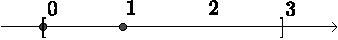
\includegraphics{figures/ode-rungeKutta05}
\[
\frac{h}{2}\left(3f\left(x_{0}+\frac{1}{3}h\right)-f(x_{0})\right)+O(h^{3})
\]
\item \label{exc:ode-rungeKutta-4}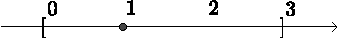
\includegraphics{figures/ode-rungeKutta06}
\[
hf\left(x_{0}+\frac{1}{3}h\right)+O(h^{2})
\]
\item \label{exc:ode-rungeKutta-5}\hasasolution 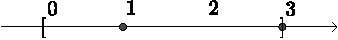
\includegraphics{figures/ode-rungeKutta07}
\[
\frac{h}{4}\left(3f\left(x_{0}+\frac{1}{3}h\right)+f(x_{0}+h)\right)+O(h^{4})
\]
\item \label{exc:ode-rungeKutta-6}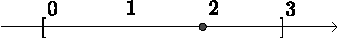
\includegraphics{figures/ode-rungeKutta08}
\[
hf\left(x_{0}+\frac{2}{3}h\right)+O(h^{2})
\]
\item \label{exc:ode-rungeKutta-7}\hasananswer 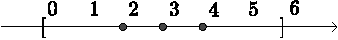
\includegraphics{figures/ode-rungeKutta09}
\[
\frac{h}{2}\left(3f\left(x_{0}+\frac{1}{3}h\right)-4f\left(x_{0}+\frac{1}{2}h\right)+3hf\left(x_{0}+\frac{2}{3}h\right)\right)+O(h^{5})
\]
\item \label{exc:ode-rungeKutta-8}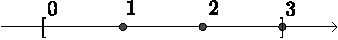
\includegraphics{figures/ode-rungeKutta10}
\[
\frac{h}{4}\left(3f\left(x_{0}+\frac{1}{3}h\right)+f(x_{0}+h)\right)+O(h^{4})
\]
\item \label{exc:ode-rungeKutta-9}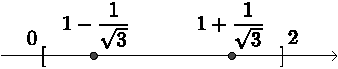
\includegraphics{figures/ode-rungeKutta11}
\[
\frac{h}{2}\left(f\left(x_{0}+\frac{\sqrt{3}-1}{2\sqrt{3}}h\right)+f\left(x_{0}+\frac{\sqrt{3}+1}{2\sqrt{3}}h\right)\right)+O(h^{5})
\]
\item \label{exc:ode-rungeKutta-10}\hasananswer 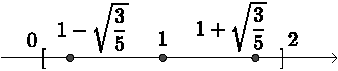
\includegraphics{figures/ode-rungeKutta12}
\[
\frac{h}{18}\left(5f\left(x_{0}+\frac{\sqrt{5}-\sqrt{3}}{2\sqrt{5}}h\right)+8f\left(x_{0}+\frac{1}{2}h\right)5f\left(x_{0}+\frac{\sqrt{5}+\sqrt{3}}{2\sqrt{5}}h\right)\right)+O(h^{7})
\]
\end{enumerate}
\item \label{exc:ode-rungeKutta-16}Lakukan eksperimen numerik pada PDB
uji \ref{eq:sampleODE} untuk menentukan laju kekonvergenan metode
yang diturunkan dalam soal \ref{exc:ode-rungeKutta}. Berdasarkan
suku galat rumus integrasi, apakah laju kekonvergenan metode penyelesaian
PDB tersebut sesuai dengan yang diharapkan?
\item \octave\ \label{exc:ode-rungeKutta-11}Tulislah fungsi Octave yang
mengimplementasikan metode Euler.  \hasananswer 
\item \octave\ \label{exc:ode-rungeKutta-12}Tulislah fungsi Octave yang
mengimplementasikan PDB-trapesium.
\item \octave\ \label{exc:ode-rungeKutta-13}Tulislah fungsi Octave yang
mengimplementasikan PDB-tertutup-terbuka.
\item \octave\ \label{exc:ode-rungeKutta-14}Tulislah fungsi Octave yang
mengimplementasikan metode penyelesaian yang Anda turunkan dalam latihan
\ref{exc:ode-rungeKutta-2}. Metode ini disebut metode titik tengah\index{metode titik tengah}\index{metode!titik tengah|see {metode titik tengah}}
atau metode Euler termodifikasi.\index{metode Euler termodifikasi}\index{metode!Euler termodifikasi|see {metode Euler termodifikasi}}
Metode ini didasarkan pada Aturan Titik Tengah untuk integrasi. \hasananswer 
\item \octave\ \label{exc:ode-rungeKutta-15}Tulislah fungsi Octave yang
mengimplementasikan metode penyelesaian yang Anda turunkan dalam latihan
\ref{exc:ode-rungeKutta-1}. Metode ini disebut metode Ralston. \hasananswer \index{metode Ralston}\index{metode!Ralston|see {metode Ralston}}
\item \octave\ \label{exc:ode-rungeKutta-17}Gunakan kode Anda dari latihan
\ref{exc:ode-rungeKutta-11} untuk menghitung $y(2)$ untuk PDB dalam
latihan \ref{exc:ode-taylor} \vpageref{exc:ode-taylor} dengan ukuran
langkah $h=0.05$.  \haspartwithsolution  \haspartwithanswer 
\item \octave\ \label{exc:ode-rungeKutta-18}Gunakan kode Anda dari latihan
\ref{exc:ode-rungeKutta-12} untuk menghitung $y(2)$ untuk PDB dalam
latihan \ref{exc:ode-taylor} \vpageref{exc:ode-taylor} dengan ukuran
langkah $h=0.05$.  \haspartwithsolution  \haspartwithanswer 
\item \octave\ \label{exc:ode-rungeKutta-19}Gunakan kode Anda dari latihan
\ref{exc:ode-rungeKutta-13} untuk menghitung $y(2)$ untuk PDB dalam
latihan \ref{exc:ode-taylor} \vpageref{exc:ode-taylor} dengan ukuran
langkah $h=0.05$.  \haspartwithsolution  \haspartwithanswer 
\item \octave\ \label{exc:ode-rungeKutta-20}Gunakan kode Anda dari latihan
\ref{exc:ode-rungeKutta-14} untuk menghitung $y(2)$ untuk PDB dalam
latihan \ref{exc:ode-taylor} \vpageref{exc:ode-taylor} dengan ukuran
langkah $h=0.05$.  \haspartwithsolution  \haspartwithanswer 
\item \octave\ \label{exc:ode-rungeKutta-21}Gunakan kode Anda dari latihan
\ref{exc:ode-rungeKutta-15} untuk menghitung $y(2)$ untuk PDB dalam
latihan \ref{exc:ode-taylor} \vpageref{exc:ode-taylor} dengan ukuran
langkah $h=0.05$.  \haspartwithsolution  \haspartwithanswer 
\end{enumerate}
\noindent\end{small} 

\subsection{Jawaban}
\begin{description}
\item [{Mengisi\ bagian\ yang\ kosong:}] \label{ans:fill-in}Dimulai
dengan rumus integrasi
\[
{\displaystyle \int_{x_{0}}^{x_{0}+3h}f(x)dx=\frac{3h}{2}\left[f(x_{0}+h)+f(x_{0}+2h)\right]+O(h^{3}f''(\xi_{h}))},
\]
kita ``perpendek'' interval integrasi menjadi $[x_{0},x_{0}+s]$
dengan melakukan substitusi $s=3h$:
\[
{\displaystyle \int_{x_{0}}^{x_{0}+s}f(x)dx=\frac{s}{2}\left[f(x_{0}+\frac{1}{3}s)+f(x_{0}+\frac{2}{3}s)\right]+O(s^{3}f''(\xi_{k}))}.
\]
Dengan menyatakan kembali rumus integrasi dalam ukuran langkah $s$,
metode penyelesaian PDB adalah
\[
y_{i+1}=y_{i}+\frac{h}{2}\left[f(t_{i+1/3},y_{i+1/3})+f(t_{i+2/3},y_{i+2/3})\right],
\]
dengan kembali menggunakan $h$ sebagai ukuran langkah. Selanjutnya,
kita menggunakan metode Euler untuk mengestimasi $y_{i+1/3}$ dan
$y_{i+2/3}$, dimulai dengan $y_{i+1/3}$. Artinya, kita mengganti
$y_{i+1/3}$ dengan $y_{i}+\frac{h}{3}f(t_{i},y_{i})$. Kemudian kita
mengestimasi $y_{i+2/3}$. Dengan perhitungan bertahap seperti sebelumnya,
kita memperoleh
\begin{eqnarray*}
k_{1} & = & f(t_{i},y_{i})\\
k_{2} & = & f\left(t_{i}+\frac{h}{3},y_{i}+\frac{h}{3}k_{1}\right),
\end{eqnarray*}
yang menangani suku pertama di dalam tanda kurung. Selanjutnya, kita
perlu mengestimasi $f(t_{i+2/3},y_{i+2/3})$. Namun, kini kita telah
memiliki estimasi untuk $f$ (turunan dari $y$) pada $t_{i}+\frac{h}{3}$,
dan $t_{i}+\frac{h}{3}$ lebih dekat ke $t_{i+2/3}$ daripada $t_{i}$.
Jadi, kita mengaproksimasi $y_{i+2/3}$ dengan $y_{i}+\frac{2}{3}hk_{2}$:
\begin{eqnarray*}
k_{1} & = & f(t_{i},y_{i})\\
k_{2} & = & f\left(t_{i}+\frac{h}{3},y_{i}+\frac{h}{3}k_{1}\right)\\
k_{3} & = & f(t_{i}+\frac{2h}{3},y_{i}+\frac{2h}{3}k_{2})\\
y_{i+1} & = & y_{i}+\frac{h}{2}\left[k_{2}+k_{3}\right].
\end{eqnarray*}
\item [{Newton-Cotes\ tertutup-terbuka:}] \label{ans:clopenNewtonCotes}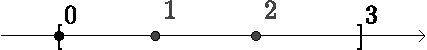
\includegraphics{figures/ode-rungekutta02}

\noindent Untuk stensil ini, $a=x_{0}$, $b=x_{0}+3h$, dan $\theta_{i}=ih$,
$i=0,1,2$. Oleh karena itu, kita akan memperoleh sistem tiga persamaan
dengan tiga variabel tak diketahui. Pertama, ruas-ruas kirinya:

\begin{eqnarray*}
\int_{a}^{b}p_{0}(x)dx=\int_{x_{0}}^{x_{0}+3h}p_{0}(x)dx & = & \int_{x_{0}}^{x_{0}+3h}1dx=\left.(x-x_{0})\right|_{x_{0}}^{x_{0}+3h}=3h\\
\int_{a}^{b}p_{1}(x)dx=\int_{x_{0}}^{x_{0}+3h}p_{1}(x)dx & = & \int_{x_{0}}^{x_{0}+3h}(x-x_{0})dx=\left.\frac{1}{2}(x-x_{0})^{2}\right|_{x_{0}}^{x_{0}+3h}=\frac{9}{2}h^{2}\\
\int_{a}^{b}p_{2}(x)dx=\int_{x_{0}}^{x_{0}+3h}p_{2}(x)dx & = & \int_{x_{0}}^{x_{0}+3h}(x-x_{0})^{2}dx=\left.\frac{1}{3}(x-x_{0})^{3}\right|_{x_{0}}^{x_{0}+3h}=9h^{3}
\end{eqnarray*}
Sekarang, kita gabungkan ruas-ruas tersebut dengan ruas-ruas kanan
(serta menukar kedua ruas):
\begin{eqnarray*}
\sum_{i=0}^{2}(\theta_{i}h)^{0}a_{i} & = & a_{0}+a_{1}+a_{2}=3h\\
\sum_{i=0}^{2}(\theta_{i}h)^{1}a_{i} & = & ha_{1}+2ha_{2}=\frac{9}{2}h^{2}\\
\sum_{i=0}^{2}(\theta_{i}h)^{2}a_{i} & = & h^{2}a_{1}+4h^{2}a_{2}=9h^{3}
\end{eqnarray*}
Sistem ini cukup kecil untuk diselesaikan secara manual (tanpa menggunakan
sistem aljabar komputer):

\begin{center}
\begin{tabular}{ccccc}
 & $h^{2}a_{1}$ & $+4h^{2}a_{2}$ & $=$ & $9h^{3}$\tabularnewline
$-$ & $(h^{2}a_{1}$ & $+2h^{2}a_{2}$ & $=$ & $\frac{9}{2}h^{3})$\tabularnewline
\hline 
 &  & $2h^{2}a_{2}$ & $=$ & $\frac{9}{2}h^{3}$\tabularnewline
\end{tabular}$\Rightarrow a_{2}=\frac{9}{4}h$.
\par\end{center}

\noindent Dengan menyubstitusikan $a_{2}=\frac{9}{4}h$ ke dalam $ha_{1}+2ha_{2}=\frac{9}{2}h^{2}$,
kita dapat menentukan $a_{1}$:
\begin{eqnarray*}
ha_{1}+2h\cdot\frac{9}{4}h & = & \frac{9}{2}h^{2}\\
ha_{1}+\frac{9}{2}h^{2} & = & \frac{9}{2}h^{2}\quad\Rightarrow a_{1}=0.\\
ha_{1} & = & 0
\end{eqnarray*}
Dengan menyubstitusikan $a_{1}=0$ dan $a_{2}=\frac{9}{4}h$ ke dalam
$a_{0}+a_{1}+a_{2}=3h$, kita dapat menentukan $a_{0}$:
\begin{eqnarray*}
a_{0}+0+\frac{9}{4}h & = & 3h\\
a_{0} & = & 3h-\frac{9}{4}h\quad\Rightarrow a_{0}=\frac{3}{4}h.
\end{eqnarray*}
Dengan demikian, $\sum_{i=0}^{2}a_{i}f(x_{0}+\theta_{i}h)=\frac{3}{4}h\cdot f(x_{0})+0\cdot f(x_{0}+h)+\frac{9}{4}h\cdot f(x_{0}+2h)$
dan rumus integrasinya adalah
\[
\int_{x_{0}}^{x_{0}+3h}f(x)dx\approx\frac{3h}{4}\left[f(x_{0})+3f(x_{0}+2h)\right].
\]

\item [{Kode\ uji:}] \label{ans:testCode}Perbandingan PDB-Simpson, PDB-terbuka,
dan PDB-tertutup-terbuka:

\begin{lyxcode}
t=4;

h=-1/4;

f=@(t,y)~-y/t+t\textasciicircum 2;

exact=@(t)~t\textasciicircum 3/4+16/t;

simp=20;

open=20;

clop=20;

disp('~~~~~~~~Simpsons~~Open~~~~~~Clopen~~~~Simp~err~~Open~err~~Clop~err')

disp('~~~~~~~~-{}-{}-{}-{}-{}-{}-{}-{}-{}-{}-{}-{}-{}-{}-{}-{}-{}-{}-{}-{}-{}-{}-{}-{}-{}-{}-{}-{}-{}-{}-{}-{}-{}-{}-{}-{}-{}-{}-{}-{}-{}-{}-{}-{}-{}-{}-{}-{}-{}-{}-{}-{}-{}-{}-{}-{}-{}-{}-{}-')

for~i=1:8

~~k1simp=f(t,simp);

~~k1open=f(t,open);

~~k1clop=f(t,clop);

~~k2simp=f(t+h/2,simp+h/2{*}k1simp);

~~k2open=f(t+h/3,open+h/3{*}k1open);

~~k2clop=f(t+h/3,clop+h/3{*}k1clop);

~~k3simp=f(t+h,simp+h{*}k2simp);

~~k3open=f(t+2{*}h/3,open+2{*}h/3{*}k2open);

~~k3clop=f(t+2{*}h/3,clop+2{*}h/3{*}k2clop);

~~simp=simp+h/6{*}(k1simp+4{*}k2simp+k3simp);

~~open=open+h/2{*}(k2open+k3open);

~~clop=clop+h/4{*}(k1clop+3{*}k3clop);

~~t=t+h;

~~x=exact(t);

~~sierr=abs(simp-x);

~~operr=abs(open-x);

~~clerr=abs(clop-x);

~~sprintf('\%12.5g\%12.5g\%12.5g\%12.5g\%12.5g\%12.5g',simp,open,clop,sierr,operr,clerr)

end\%for
\end{lyxcode}
Kode uji ini dapat diunduh di \href{http://lqbrin.github.io/tea-time-numerical/ancillaries.html}{situs pendamping}
(\texttt{rungeKuttaDemo2.m}). 
\item [{Suku\ galat:}] \label{ans:errorTerms}Suku galat untuk
\[
\int_{x_{0}}^{x_{0}+3h}f(x)dx\approx\frac{3h}{4}\left[f(x_{0})+3f(x_{0}+2h)\right]
\]
diturunkan dalam jawaban untuk Bagian \ref{sec:calculusErrorAnalysis}.
Lihat halaman \pageref{sol:exc:calculusErrors-11}. Suku galat untuk
\[
\int_{x_{0}}^{x_{0}+h}f(x)dx\approx hf(x_{0})
\]
diturunkan dengan cara serupa. Diketahui bahwa galatnya adalah $O(h^{2})$,
sehingga kita dapat melewati proses penurunannya. Dengan mengembangkan
$f(x)$ dalam polinomial Taylor dengan suku galat,
\[
f(x)=f(x_{0})+(x-x_{0})f'(\xi_{x}).
\]
Dengan demikian,
\begin{eqnarray*}
\int_{x_{0}}^{x_{0}+h}f(x)dx-hf(x_{0}) & = & \int_{x_{0}}^{x_{0}+h}\left(f(x_{0})+(x-x_{0})f'(\xi_{x})\right)dx-hf(x_{0})\\
 & = & \left.xf(x_{0})\right|_{x_{0}}^{x_{0}+h}+\int_{x_{0}}^{x_{0}+h}(x-x_{0})f'(\xi_{x})dx-hf(x_{0})\\
 & = & hf(x_{0})+\int_{x_{0}}^{x_{0}+h}(x-x_{0})f'(\xi_{x})dx-hf(x_{0})\\
 & = & \int_{x_{0}}^{x_{0}+h}(x-x_{0})f'(\xi_{x})dx.
\end{eqnarray*}
Menurut Teorema Nilai Rata-Rata Berbobot, terdapat $c\in(x_{0},x_{0}+h)$
sedemikian sehingga $\int_{x_{0}}^{x_{0}+h}(x-x_{0})f'(\xi_{x})dx=f'(c)\int_{x_{0}}^{x_{0}+h}(x-x_{0})dx=\frac{1}{2}f'(c)h^{2}$.
Oleh karena itu, 
\[
\int_{x_{0}}^{x_{0}+h}f(x)dx-hf(x_{0})=\frac{1}{2}f'(c)h^{2}\leq Mh^{2}f'(\xi_{h})
\]
dengan mengganti $c$ dengan $\xi_{h}$. 
\end{description}

